% !TeX root = ../paper.tex
\begin{figure}[!t]
  \centering
  \setlength{\parskip}{0pt}
  \setlength{\abovecaptionskip}{\baselineskip}
  \setlength{\belowcaptionskip}{0pt}
  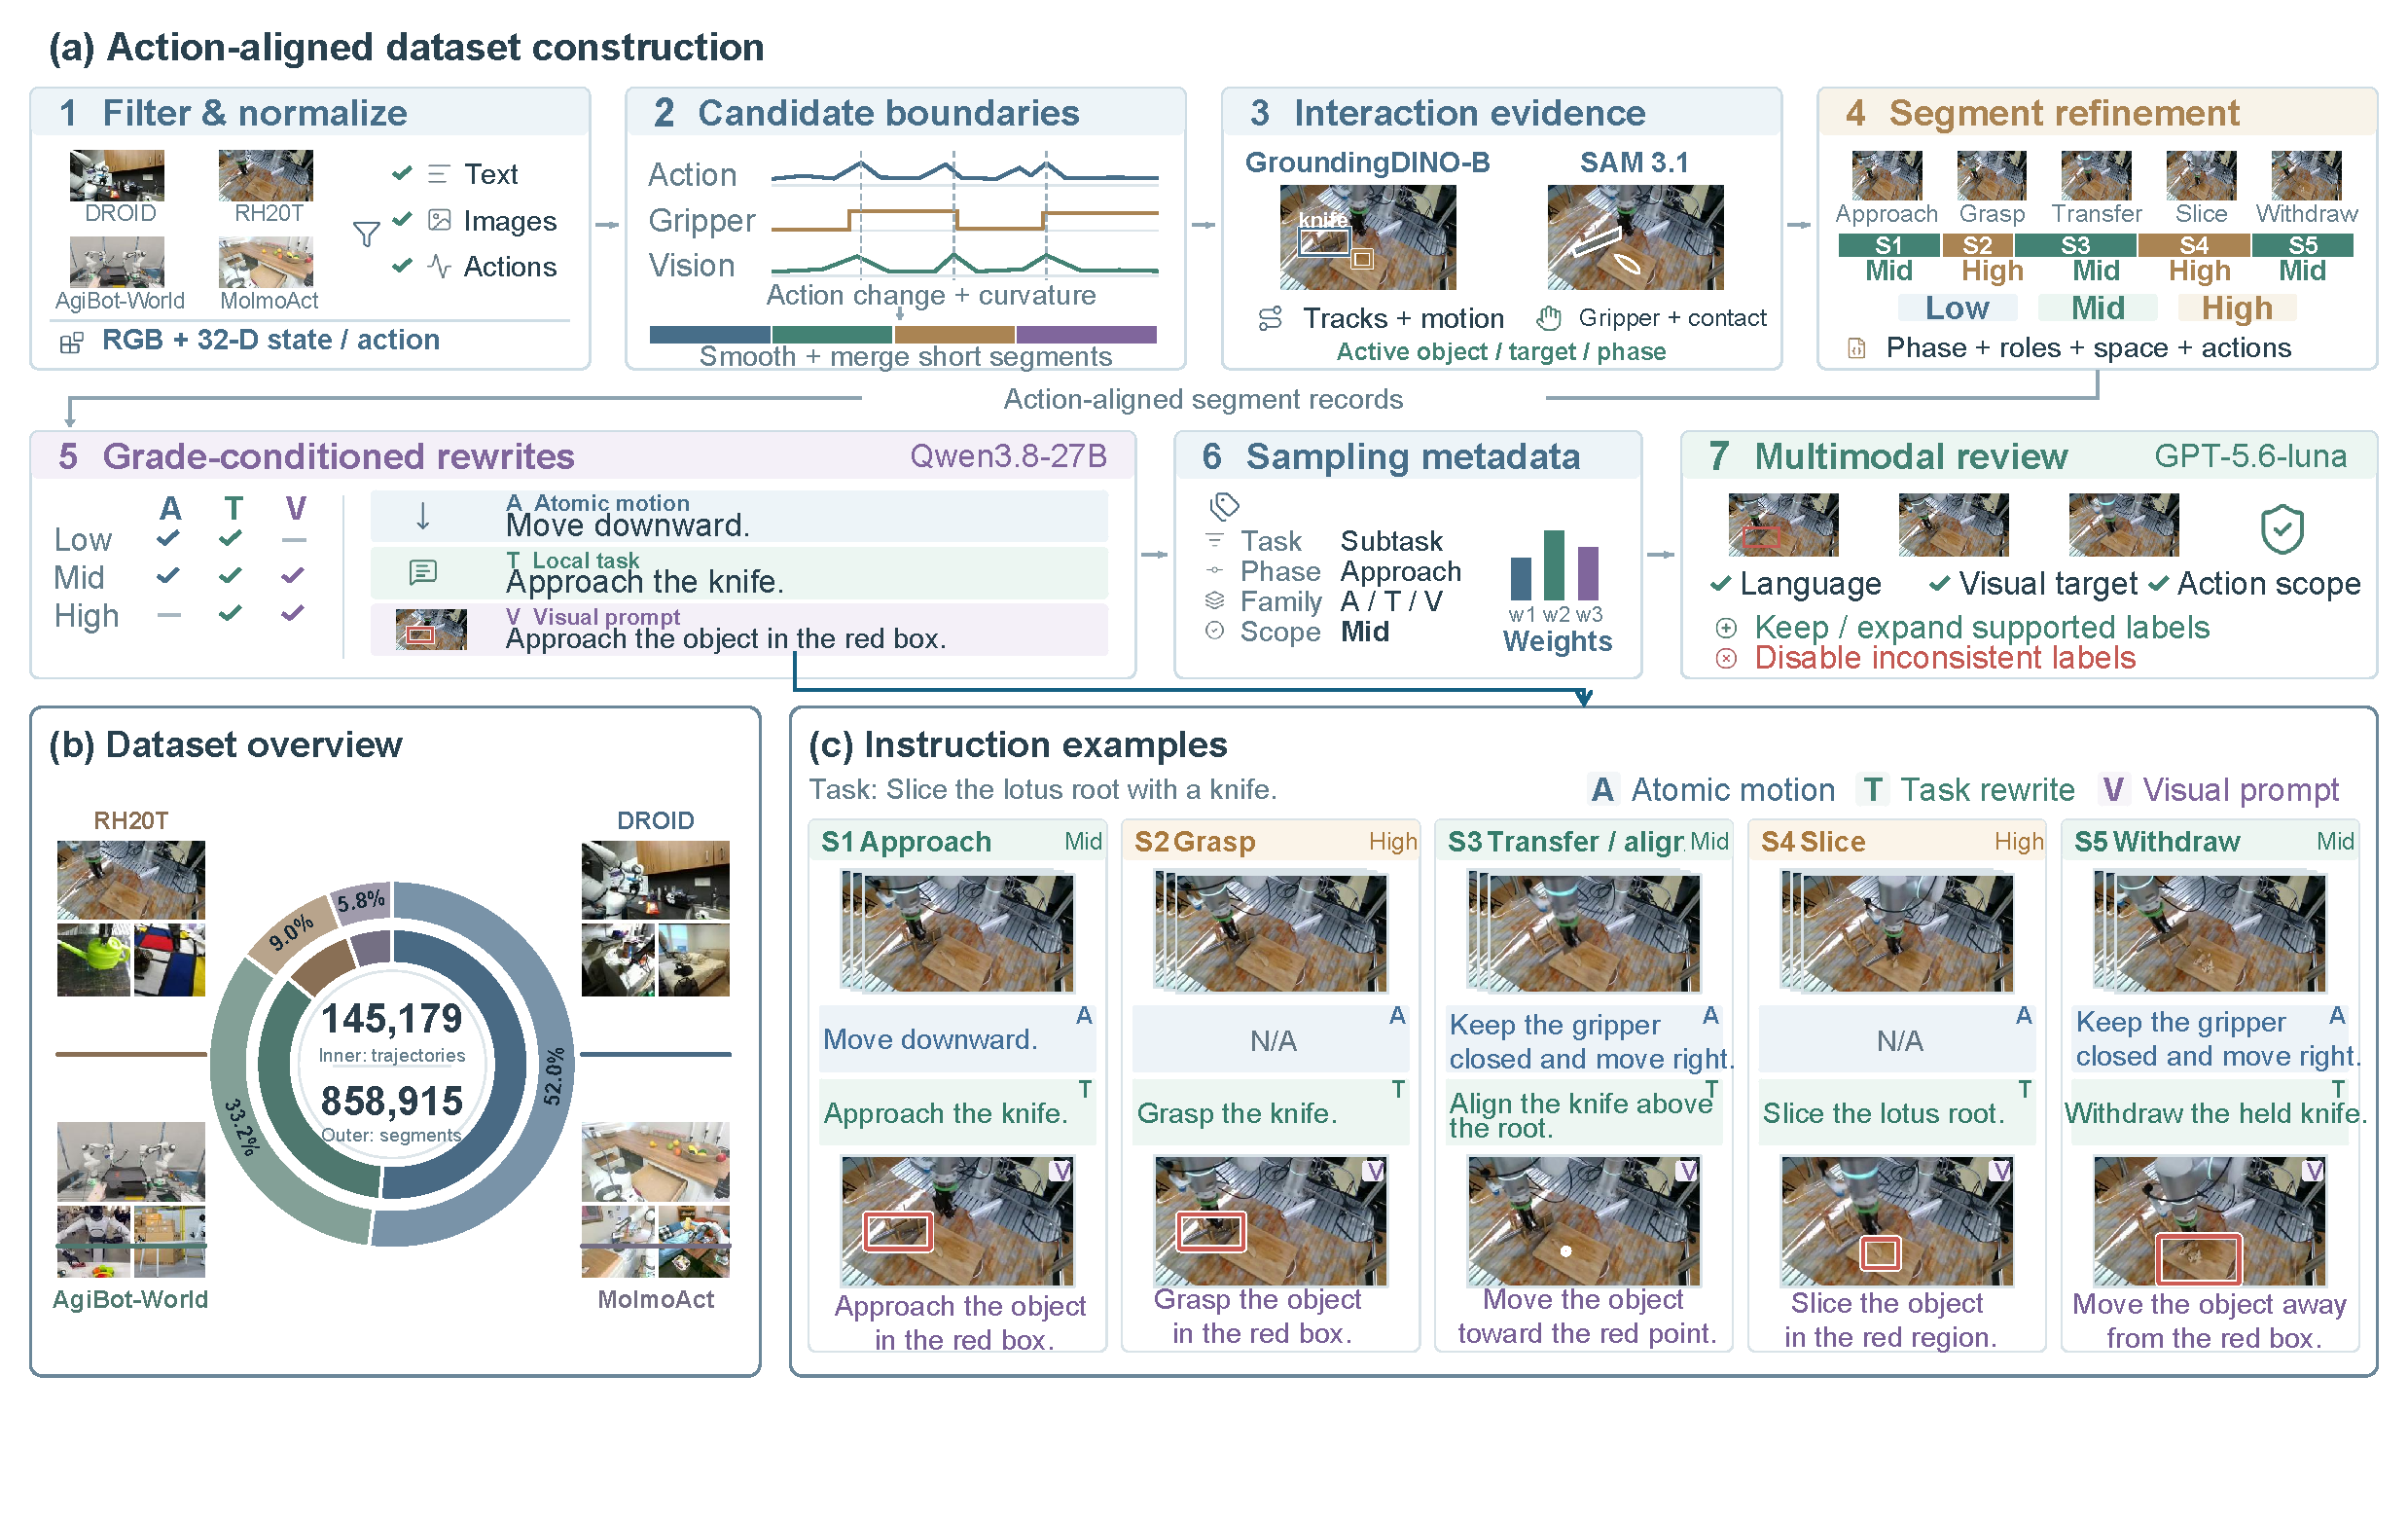
\includegraphics[width=\textwidth,pagebox=cropbox]{figures/datasets.pdf}\par\nointerlineskip
  \caption{Action-aligned data construction and supervision. (a) Seven-stage pipeline from raw
  demonstrations to reviewed segment annotations. (b) Source composition of the retained
  trajectories (inner ring) and action segments (outer ring). (c) Grade-conditioned atomic-motion
  (A), task-language (T), and visual-prompt (V) examples from an RH20T demonstration; N/A denotes an
  inapplicable rewrite family.}
  \label{fig:dataset-construction}
\end{figure}
